\scanpage{65}

\diagram{\begin{tikzcd}
\underline O_{\hat C}(\unsure{U|1})\arrow[r,rightsquigarrow]&
\underline O_{\hat C_X}(\unsure{U|1})
\end{tikzcd}}
\[
\hat C=\operatorname{Spec}S[z]\qquad
\left\{\begin{gathered}\text{induit }0\\\text{sur }C\text{ et}\\\text{sur }C'\end{gathered}\right.
\]
\[
O_{\hat C}(1)
\]

\diagram{\begin{tikzcd}
\operatorname{Pic}(\hat C)\arrow[r]&{}
\end{tikzcd}}

\margin{\deleted{\unsure{Pic $C$}}}

\diagram{\begin{tikzcd}[column sep=large,row sep=large]
\operatorname{Pic}(X)
\arrow[r,"{\text{injectif,}}","{\substack{[\text{bijectif}\\\text{dans le cas}\\X\ \unsure{\text{loc.}}\ \text{factoriel}]}}"']
\arrow[rr,bend left=30,"{\text{noyau }\unsure{\subset\underline{Z\xi}|\text{engendré}}}"]&
\operatorname{Pic}(\hat C')\arrow[r]
\arrow[dr]&
\operatorname{Pic}(C')\arrow[r,"{\text{injectif}}"',"{\substack{[\text{surjectif}\\\text{dans le}\\\unsure{\text{cas local}}\\\text{factoriel}]}}"]&
\operatorname{Pic}(\widetilde C')\\
&&\substack{\text{noyau}\\{}[\text{engendré par}\\\text{l'image de }O_X(1)}&
\end{tikzcd}}

\[
\operatorname{Pic}(X)/Z.\unsure{\xi|\zeta}\ \subset\
\operatorname{Pic}(\hat C')/Z\unsure{\xi|\zeta})
\]

\margin{\figure{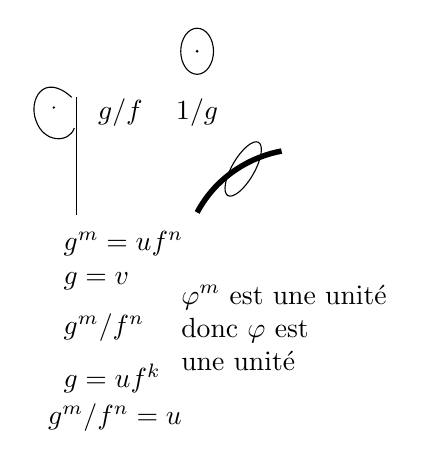
\begin{tikzpicture}[x=.65cm,y=.65cm]
\draw (-.35,3.7) -- (-.35,1.4);
\draw[thin] (-.45,3.7) .. controls (-1,4.2) and (-1.3,3.65) .. (-1.15,3.25)
 .. controls (-1,2.8) and (-.5,2.8) .. (-.4,3.1);
\fill (-.8,3.5) circle (.025);
\draw[thin] (2,4.6) ellipse (.32 and .45);
\fill (2,4.6) circle (.03);
\node at (.5,3.4) {$g/f$};
\node at (2,3.4) {$1/g$};
\draw[line width=2pt] (2,1.45) .. controls (2.4,2.2) and (3.1,2.55) .. (3.65,2.65);
\draw[thin,rotate around={-30:(2.9,2.3)}] (2.9,2.3) ellipse (.22 and .6);
\node[anchor=west] at (-.8,.85) {$g^m=uf^n$};
\node[anchor=west] at (-.8,.1) {$\deleted{g=\unsure{v}}$};
\node[anchor=west] at (-.8,-.8) {$\deleted{\unsure{g^m/f^n}}$};
\node[anchor=west] at (-.8,-1.8) {$g=uf^k$};
\node[anchor=west] at (-1.1,-2.55) {$\unsure{g^m/f^n=u}$};
\node[align=left,anchor=west] at (1.5,-.8)
 {$\varphi^m$ est une unité\\donc $\varphi$ est\\une unité};
\end{tikzpicture}}}

\figure{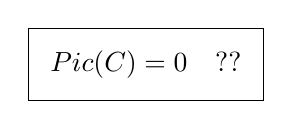
\begin{tikzpicture}
\node[draw,rectangle,inner sep=8pt] {$\operatorname{Pic}(C)=0\quad??$};
\end{tikzpicture}}

\diagram{\begin{tikzcd}[column sep=large,row sep=large]
&&0\arrow[d]&\\
&Z.\unsure{\xi|\zeta}\arrow[r,dash]\arrow[d]&Z\unsure{\xi|\zeta}
\arrow[d,"{\text{\textcircled{?}}}"]&\\
\unsure{0|\bullet}\arrow[r,dash]&\operatorname{Pic}(X)
\arrow[r,"{\substack{\text{injectif}\\{}[\text{surjectif}]}}"']&
\operatorname{Pic}(\hat C')
\arrow[d,"{\substack{\deleted{\text{injectif}}\\{}[\text{surjectif}]}}"]&
\unsure{\mathbin{-}}\arrow[l]\\
&\operatorname{Pic}(C)\arrow[r]&\operatorname{Pic}(C')\arrow[r]&
\operatorname{Pic}(\widetilde C')
\end{tikzcd}}

\margin{$\unsure{1|\downarrow}$}

\margin{\figure{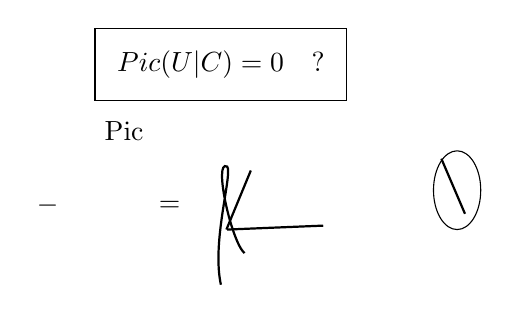
\begin{tikzpicture}
\node[draw,rectangle,inner sep=8pt] at (0,1.7) {$\operatorname{Pic}(\unsure{U|C})=0\quad?$};
\node[anchor=west] at (-1.6,.85) {Pic};
\node at (-2.2,-.1) {$-$};
\node at (-.65,-.1) {$=$};
\draw[thick] (0,-1.1) .. controls (-.12,-.55) and (.15,.3) .. (.08,.4)
 .. controls (-.1,.5) and (.13,-.55) .. (.3,-.7);
\draw[thick] (.07,-.4) -- (.38,.35);
\draw[thick] (.08,-.4) -- (1.3,-.35);
\draw[thin] (3,.1) ellipse (.3 and .5);
\draw[thick] (2.8,.5) -- (3.1,-.2);
\end{tikzpicture}}}

\figure{
\begin{tikzpicture}[x=1cm,y=1cm]
\draw[thin] (0,1) .. controls (.6,.65) and (1.1,.3) .. (1.2,-1);
\draw[thin] (-.1,-.65) .. controls (.65,-.4) and (.9,.1) .. (1.15,.9);
\fill (.75,.2) circle (.025);
\draw[thin] (3,.85) -- (4.2,.6);
\draw[thin] (3.6,1) .. controls (3.2,.2) and (3.35,-.4) .. (3.55,-1);
\draw[thin] (3.85,.7) -- (3,-.5);
\fill (3.42,.1) circle (.02);
\end{tikzpicture}}

\margin{64}
